\documentclass[11pt,a4paper]{article}
\usepackage{tikz}
\usetikzlibrary{angles,quotes}

\usepackage{amsmath}
\usepackage{amsfonts}
\usepackage{amssymb}
\usepackage{graphicx}
\usepackage[left=2cm,right=2cm,top=2cm,bottom=2cm]{geometry}
\usepackage{multicol}
\usepackage{float}
\restylefloat{table}

\newcommand\Base[1][0]{
\begin{scope}[xshift=#1]
\clip
  (-0.5,5.5) rectangle (5.5,-0.5);
  \draw[->]
  (-0.5,0) -- (5,0) node[right] {$u$};
\draw[->]
  (0,-0.5) -- (0,5) node[above] {$v$};
\coordinate (O) at (0,0) node[above left] {$O$};
\coordinate (aux1) at (40:4);
\coordinate (aux2) at (aux1|-0,0);
\coordinate (aux3) at (4,{4*tan(40)});
\node at (4.2, 0.2) {$A$};
\node at (3.1, 3) {$B$};
\node at (4.2, 3.7) {$C$};
\draw
  (O) -- (aux3) -- (aux3|-0,0)
  (aux1) -- (aux2);
\draw[thick,red!70!black] 
  (O) circle (4);
\pic[draw,"$x$",angle radius=30pt,angle eccentricity=1.2] {angle = aux2--O--aux1};   
\end{scope}  
}

\author{Iker M. Canut}
\title{Unidad 3: L\'imite y Continuidad\\ Analisis Matem\'atico I}

\newcommand*{\QEDA}{\null\nobreak\hfill\ensuremath{\blacksquare}}
\newcommand*{\QEDB}{\null\nobreak\hfill\ensuremath{\square}}

\begin{document}
\maketitle
\newpage

\section{Distancia de Puntos y Entornos}
Para $x,y \in \mathbb{R}$, la \textbf{distancia} entre $x$ e $y$ es $d(x,y) = |x-y|$\\

Llamamos \textbf{entorno} de un real $a$, de radio $\delta$ al intervalo abierto $(a-\delta, a+\delta)$ y lo notamos\\ $E(a,\delta) = \{x\in\mathbb{R}:a-\delta<x<a+\delta\} = \{x\in\mathbb{R}:-\delta<x-a<\delta\} = \{x\in\mathbb{R}:|x-a|<\delta\}$

Llamamos \textbf{entorno reducido} de un real $a$, de radio $\delta$ al conjunto $E(a,\delta) - \{a\}$ y lo notamos $E'(a,\delta) = \{x\in\mathbb{R}:|x-a<\delta\land x\not = a|\} = \{x\in\mathbb{R}:0<|x-a|<\delta\}$\\

Sea $a$ un real, $\delta_1, \delta_2$ dos reales positivos, y $\delta\leq min\{\delta_1, \delta_2\}$, se tiene que:
\begin{table}[h]
\centering
\begin{tabular}{ccc}
$E(a,\delta) \subseteq E(a,\delta_1) \cap E(a,\delta_2)$ & \ \ \ \ & $E'(a,\delta) \subseteq E'(a,\delta_1) \cap E'(a,\delta_2)$\\
$|x-a|<\delta \Rightarrow |x-a|<\delta_1 \land |x-a|<\delta_2 \hfill$ & \ y \ & $\hfill 0<|x-a|<\delta \Rightarrow 0<|x-a|<\delta_1 \land 0<|x-a|<\delta_2$
\end{tabular}
\end{table}

\section{L\'imite Finito en un Punto}
Dada una funci\'on real $f$ y un real $a$, tal que $f$ est\'a definida en un entorno reducido del punto $a$, decimos que $l$ es el l\'imite de la funci\'on $f$, cuando la variable independiente tiende al valor $a$ y notamos $$\lim_{x\to a}f(x)=l$$ si para cualquier valor $\epsilon > 0$, prefijado, existe un n\'umero positivo $\delta$ tal que: $$0<|x-a|<\delta \Rightarrow |f(x)-l| < \epsilon$$ $$x \in E'(a, \delta) \Rightarrow f(x) \in E(l, \epsilon)$$ $$\forall \epsilon > 0, \exists \delta > 0 /\ \forall x : (0 < |x-a| < \delta \Rightarrow |f(x)-l|<\epsilon)$$\\

No se exige que $a$ est\'e en el dominio de $f$, pero si que $f$ este definida en un entorno reducido de $a$.\\
La siguiente simbolog\'ia es equivalente:
\begin{table}[h]
\centering
\begin{tabular}{ccc}
$\displaystyle{\lim_{x\to a}f(x)=l}$ \ \ & \ \ $\displaystyle{\lim_{x\to 0}f(x+a)=l}$ \ \ & \ \ $\displaystyle{\lim_{x\to a}f(x) - l =0}$
\end{tabular}
\end{table}

Por \'ultimo, observamos que el n\'umero $\delta$ depende tanto del valor de $\epsilon$ como del punto $a$. Adem\'as, si en un punto $a$, para un $\epsilon$, un n\'umero $\delta$ satisface la definici\'on de l\'imite, entonces cualquier $\delta'<\delta$ tambien es v\'alido. Por otro lado, si un $\delta$ es \'util para un $\epsilon$, tambi\'en es \'util para un $\epsilon' > \epsilon$. $$0 < |x-a| < \delta' \Rightarrow 0 < |x-a| < \delta \Rightarrow |f(x)-l| < \epsilon < \epsilon'$$

\section{L\'imites Finitos}
\subsection{Funci\'on Constante}
$f(x)=c \in \mathbb{R}$, $\displaystyle{\lim_{x\to a}c=c}$, pues cualquier $\epsilon > 0$ y $\delta > 0$, se verifica que $$0<|x-a|<\delta \Rightarrow |f(x)-c| = |c-c| = 0 < \epsilon$$

\subsection{Funci\'on Lineal}
$f(x)=mx+h, m \not = 0$, $\displaystyle{\lim_{x\to a}mx+h=ma+h}$
$$\forall\epsilon>0,\ \exists\delta>0:\ \forall x: (0<|x-a|<\delta \Rightarrow |f(x)-l|<\epsilon)$$
$$|(mx+h)-(ma+h)| = |m|\cdot|x-a| < \epsilon \Rightarrow |x-a| < \delta < \dfrac{\epsilon}{|m|}$$
Y considerando $\delta < \dfrac{\epsilon}{|m|}$ tenemos que $0<|x-a|<\delta<\dfrac{\epsilon}{|m|} \Rightarrow |(mx+h)-(ma+h)|=|m|\cdot|x-a| < \epsilon$

\subsection{Funci\'on Cuadratica}
$f(x)=x^2$, $\displaystyle{\lim_{x\to a}x^2=a^2}$ hay que demostrar $\forall\epsilon>0,\ \exists\delta>0:\ \forall x: (0<|x-a|<\delta \Rightarrow |x^2-a^2|<\epsilon)$
Se ve que $|x^2-a^2| = |x-a|\cdot|x+a|$
\begin{itemize}
\item Caso $a=0$: $\forall\epsilon>0,\ \exists\delta>0:\ \forall x: (0<|x|<\delta \Rightarrow |x^2|<\epsilon)$\\
Luego $|x^2|<\epsilon \iff |x|^2<\epsilon \iff |x|<\sqrt{\epsilon}$ y tenemos que: $$0<|x|<\delta=\sqrt{\epsilon} \Rightarrow |x|^2<\epsilon \Rightarrow |x^2|<\epsilon$$
\item Caso $a\not = 0$: $\forall\epsilon>0,\ \exists\delta>0:\ \forall x: (0<|x-a|<\delta \Rightarrow |x-a|\cdot|x+a|<\epsilon)$ \hfill \textbf{(1)}\\
Hay que acotar $|x+a|$. Sea $0<\delta<|a|$, \hfill \textbf{(2)}
\begin{align*}
|x-a|<\delta &\Rightarrow -|a|<-\delta<x-a<\delta<|a| \Rightarrow -|a|+2a<-\delta+2a < x+a < \delta+2a < |a|+2a\\
& \Rightarrow -|a|-2|a| < x+a < |a|+2|a| \Rightarrow |x+a| < 3|a|
\end{align*}
Y tenemos que $|x-a|<\delta \Rightarrow |x+a| < 3|a|$. \hfill \textbf{(3)}\\
De \textbf{(2)} para que se verifique \textbf{(3)} y de \textbf{(1)} tenemos que $\delta\leq min\left\{|a|, \dfrac{\epsilon}{3|a|}\right\}$\\
Luego, $|x-a|<\dfrac{\epsilon}{3|a|} \land |x+a|<3|a|$. Y tenemos que $$0<|x-a|<\delta \Rightarrow |x^2-a^2| = |x-a|\cdot|x+a| < \dfrac{\epsilon}{3|a|}\cdot 3|a| = \epsilon$$
\end{itemize}

\subsection{Funci\'on Reciproca}
$f(x)=\dfrac{1}{x}$, $\displaystyle{\lim_{x\to a}\dfrac{1}{x}=\dfrac{1}{a}}$ hay que demostrar $\forall\epsilon>0,\ \exists\delta>0:\ \forall x: (0<|x-a|<\delta \Rightarrow |\dfrac{1}{x}-\dfrac{1}{a}|<\epsilon)$\\

\indent Se demuestra fijando un $\epsilon$ a cualquier n\'umero. Despu\'es se calcula la otra parte del m\'inimo.

\section{Unicidad del L\'imite}
\noindent \textbf{Teorema 1}: \textbf{Unicidad del L\'imite}. Sea $f$ una funci\'on real definida en un entorno reducido del punto $a$ y sean $l_1$ y $l_2$ dos n\'umeros reales tales que: \ \ $\displaystyle{\lim_{x\to a}f(x)=l_1} \ \land \ \displaystyle{\lim_{x\to a}f(x)=l_2} \ \ \Rightarrow \ \ \ \ l_1 = l_2$\\
\textbf{Demostraci\'on: } Dado $\epsilon > 0$, tenemos $\delta_1$ y $\delta_2$ tales que: $$0 < |x-a| < \delta_1 \Rightarrow |f(x) - l_1| < \dfrac{\epsilon}{2} \ \ \land \ \ 0 < |x-a| < \delta_2 \Rightarrow |f(x) - l_2| < \dfrac{\epsilon}{2}$$
Considerando $\delta = \min\{\delta_1, \delta_2\}$, considerando cualquier $E'(a, \delta)$, tenemos que:
$$|l_1 - l_2| = |l_1 - f(x) + f(x) - l_2| \leq |l_1 - f(x)| + |l_2 - f(x)| < \dfrac{\epsilon}{2} + \dfrac{\epsilon}{2} = \epsilon$$
Y como tenemos $0 \leq |l_1 - l_2| < \epsilon$, podemos asegurar que $|l_1 - l_2| = 0 \Rightarrow l_1 = l_2$ \QEDA

\section{No Existencia de L\'imite}
Negando la forma proposicional de la definici\'on de l\'imite, llegamos a que no existe el l\'imite si: $$\exists \epsilon > 0 /\ \forall \delta > 0, \exists x: (0< |x-a| < \delta \land |f(x) - l| \geq \epsilon)$$
Generalmente se demuestra que un $l=b$ no es l\'imite (fijo), y que $l \not = b$ tampoco lo es (relaci\'on a $l$).

\section{L\'imites Laterales}
$$\lim_{x \to a^+} f(x) = l, \text{ si } \forall \epsilon > 0,\ \exists \delta > 0: a < x < a+\delta \Rightarrow |f(x)-l| = \epsilon$$
$$\lim_{x \to a^-} f(x) = l, \text{ si } \forall \epsilon > 0,\ \exists \delta > 0: a-\delta < x < a \Rightarrow |f(x)-l| = \epsilon$$\\

\noindent \textbf{Proposici\'on 1}: $\displaystyle{ \lim_{x \to a} f(x) = l \iff \lim_{x \to a^-} f(x) = l \land \lim_{x \to a^+} f(x) = l}$\\
\noindent \textbf{Demostraci\'on}:\\ $\Rightarrow)$ Si $\forall \epsilon > 0,\ \exists \delta > 0:\ \forall x: (0<|x-a|<\delta \Rightarrow |f(x)-l|<\epsilon$\\
Para ese $\delta$ se verifica \ $a-\delta<x<a \Rightarrow 0<|x-a|<\delta \Rightarrow |f(x)=l| \therefore \text{ Existe el l\'imite por izquierda.}$\\
\indent \indent \indent \indent \indent \ \ \ \ \ \ $a<x<a+\delta \Rightarrow 0<|x-a|<\delta \Rightarrow |f(x)=l| \therefore \text{ Existe el l\'imite por derecha.}$ \\
\QEDB\\
$\Leftarrow)$ Si $\forall \epsilon > 0, \exists \delta_1, \delta_2$ tales que: \ \
$a-\delta_1 < x < a \Rightarrow |f(x)-l| < \epsilon \ \ \ \ \land \ \ \ \ a<x<a+\delta \Rightarrow |f(x)-l| < \epsilon$\\
Sea $\delta=\min{\delta_1, \delta_2}$:\\
$a-\delta<x<a \Rightarrow a-\delta_1<x<a \Rightarrow |f(x)-l| < \epsilon \ \ \land \ \ a<x<a+\delta \Rightarrow a<x<a+\delta_2 \Rightarrow |f(x)-l|<\epsilon$\\
$\Rightarrow 0<|x-a|<\delta \Rightarrow |f(x)-l| < \epsilon \therefore \displaystyle{\lim_{x \to a} f(x) = l}$\\
\QEDA \\
\textit{Nota: Como la existencia e igualdad de l\'imites laterales en un punto es condici\'on necesaria y suficiente para garantizar la existencia de l\'imites alli, la no existencia de alguno de los l\'imites laterales, o la diferencia entre ambos, implica la no existencia de l\'imites finito de la funci\'on en el punto.}\\

\noindent \textbf{Proposici\'on 2}: Sea $f$ una funci\'on y $a$ un numero tal que existe $\displaystyle{\lim_{x\to a}f(x) = l} \Rightarrow \lim_{x\to a}|f(x)|=|l|$\\
\textbf{Demostraci\'on}: Dado $\epsilon > 0,\ \exists \delta > 0 : (0<|x-a|<\delta \Rightarrow |f(x)-l)<\epsilon)$\\
Y como $||f(x)|-|l|| < |f(x)-l|$, para el mismo $\delta$: $(0<|x-a|<\delta \Rightarrow ||f(x)|-|l|| < |f(x)-l)<\epsilon)$\\ \QEDA \\

\noindent \textbf{Teorema 2}: \textbf{Caracter Local del L\'imite}: Sean $a$ un real, y dos funciones $f$ y $g$ para las cuales:
$$\lim_{x\to a}f(x) = l \ \ \land \ \ f(x) = g(x) \text{ en alg\'un } E'(a, \rho) \ \ \Rightarrow \ \ \lim_{x\to a}g(x) = l$$
\textbf{Demostraci\'on}: Dado $\epsilon>0, \exists \delta'>0 : (0<|x-a|<\delta' \Rightarrow |f(x)-l|<\epsilon)$\\
Por Hipotesis, existe $\rho > 0$ tal que $0<|x-a|<\rho \Rightarrow f(x)=g(x)$, y eligiendo $\delta = \min\{\delta', \rho\}$, vale:
$$0<|x-a|<\delta \Rightarrow |f(x)-l|<\epsilon \ \ \land \ \ f(x)=g(x) \Rightarrow |g(x)-l|<\epsilon \ \ \therefore \ \ 0<|x-a|<\delta \Rightarrow |g(x)-l|<\epsilon$$ \QEDA \\

\noindent \dotfill\\

Sea $A$ un subconjunto no vacio de $\mathbb{R}$ y $f$ una funci\'on definida en $A$, diremos que la funci\'on $F$ est\'a \textbf{acotada} en el conjunto $A$ si existe un n\'umero real $M > 0$ tal que $\forall x \in A$: $|f(x)| \leq M$.\\
\indent De manera alternativa, $f$ est\'a acotada en $A$ si $\{f(x):x\in A\}$ es un subconjunto acotado de $\mathbb{R}$.\\

\noindent \textbf{Teorema 3}: Si tenemos que $\displaystyle{\lim_{x\to a}f(x) = l}$, entonces existe $E'(a,\delta)$ en el cual la funci\'on est\'a acotada.\\
\noindent \textbf{Demostraci\'on}: Dado, por ejemplo, $\epsilon=1$, existe $\delta>0 : x\in E'(a,\delta) \Rightarrow |f(x)-l|<1$. Luego, 
\begin{align*}
|f(x)-l| < 1 & \Rightarrow -1 < f(x)-l < 1 \Rightarrow l-1<f(x)<l+1\\
& \Rightarrow -|l|-1 \leq l-1<f(x)<l+1\leq|l|+1\\
& \Rightarrow -(|l|+1) < f(x) < (|l|+1) \Rightarrow |f(x)|<|l|+1
\end{align*}
\QEDA\\

La rec\'iproca no necesariamente es cierta, hay funciones acotadas en todo entorno reducido de $a$ que no tienen l\'imite en $a$ (e.g signo en $a=0$).

\newpage

\noindent \textbf{Teorema 4}: Si tenemos que $\displaystyle{\lim_{x\to a}f(x) = l}$ y dos n\'umeros $k$ y $h$, tales que $h<l<k$,\\
entonces existe un entorno reducido $E'(a,\delta)$ donde, $\forall x \in E'(a,\delta)$, se verifica $h < f(x) < k$.\\
\textbf{Demostraci\'on}: \\
Siendo $l < k$, eligiendo $\epsilon = k - l > 0$, sabemos que existe $\delta_1 > 0$ tal que\\ si $x\in E'(a,\delta_1) \Rightarrow |f(x)-l|<k-l$. Y en ese entorno, $f(x)-l \leq |f(x)-l| < k-l \therefore f(x) < k$ \hfill \textbf{(1)}\\
Siendo $h < l$, eligiendo $\epsilon = l - h > 0$, sabemos que existe $]dekta_2 > 0$ tal que\\ si $x\in E'(a,\delta_2) \Rightarrow |f(x)-l|<l-h$. Y en ese entorno, $h-l<f(x)-l<l-h \therefore h<f(x)$ \hfill \textbf{(2)}\\
Considerando $\delta=\min\{\delta_1,\delta_2\}$, vale de \textbf{(1)} y \textbf{(2)} que $x\in E'(a,\delta) \Rightarrow h < f(x) < k$\\
\QEDA\\

\noindent \textbf{Corolario 1}: \textbf{Teorema de Conservaci\'on del Signo}. Si tenemos que $\displaystyle{\lim_{x\to a}f(x) = l \not = 0}$, entonces existe un entorno reducido $E'(a,\delta)$ donde $f(x)\not = 0$. Y vale, por ejemplo, $|f(x)| > \frac{|l|}{2}$\\
\noindent \textbf{Demostraci\'on}: Teorema anterior. Si $l<0, h=\dfrac{l}{2}<l$. Si $l>0, k=\dfrac{l}{2}>l$. Por la proposici\'on 2, vale $\displaystyle{\lim_{x\to a}|f(x)| = |l| \not = 0}$\\
\QEDA\\

\section{\'Algebra de L\'imites}
\noindent \textbf{Teorema 5}: Sea $a$ un real, $f$ y $g$ dos funciones tales que $\displaystyle{\lim_{x\to a}f(x) = l_1}$ y $\displaystyle{\lim_{x\to a}g(x) = l_2}$, entonces:
\begin{itemize}
\item $\displaystyle{\lim_{x\to a}(f+g)(x) = l_1 + l_2}$\\
\textbf{Dem}: $0<|x-a|<\delta_1 \Rightarrow |f(x)-l_1| < \dfrac{\epsilon}{2}$ y $0<|x-a|<\delta_2 \Rightarrow |g(x)-l_2| < \dfrac{\epsilon}{2}$\\
Sea $\delta=\min\{\delta_1, \delta_2\}$, y $x$ tal que $0<|x-a|<\delta$,\\
$|(f+g)(x)-(l_1+l_2)| = |(f(x)-l_1)+(f(x)-l_2)| \leq |f(x)-l_1| + |f(x)-l_2| < \dfrac{\epsilon}{2} + \dfrac{\epsilon}{2} = \epsilon$\\
\QEDA
\item Sea $c\in \mathbb{R}$, $\displaystyle{\lim_{x\to a}(c\cdot f)(x) = c\cdot l_1}$\\
\textbf{Dem}: Si $c=0$ es trivial. Sea $c\not = 0$, dado $\epsilon > 0$, sea $\delta > 0$ : $0<|x-a|<\delta \Rightarrow |f(x)-l_1| < \dfrac{\epsilon}{|c|}$.\\
Entonces para los $x$ : $0<|x-a|<\delta$, $|(c\cdot f)(x) - (c\cdot l_1)| = |c \cdot (f(x)-l_1)| = |c|\cdot|f(x)-l_1| < |c|\cdot\dfrac{\epsilon}{|c|}=\epsilon$\\
\QEDA
\item $\displaystyle{\lim_{x\to a}(f-g)(x) = l_1 - l_2}$\\
\textbf{Dem}: $\displaystyle{\lim_{x\to a}(f-g)(x) = \lim_{x\to a}(f+ (-1)g)(x) = \lim_{x\to a}f(x) + (-1)\lim_{x\to a}g(x) = l_1 - l_2}$\\
\QEDA
\end{itemize}
\noindent \dotfill\\

\noindent \textbf{Teorema 6}: Si $\displaystyle{\lim_{x\to a}f(x) = 0}$ y $g$ est\'a acotada en un entorno reducido $E'(a,\rho)$, entonces $\displaystyle{\lim_{x\to a}(fg)(x) = 0}$\\
\noindent \textbf{Demostraci\'on}: Tenemos que $0<|x-a|<\delta' \Rightarrow |f(x)|<\dfrac{\epsilon}{M}$ y $0<|x-a|<\rho \Rightarrow |g(x)| \leq M$.\\
Luego, considerando $\delta = \min\{\delta', \rho\}$, y $x$ tal que $0<|x-a|<\delta$, $$|(f\cdot g)(x)-0| = |f(x)\cdot g(x)| = |f(x)|\cdot|g(x)| < \dfrac{\epsilon}{M} \cdot M = \epsilon$$
\QEDA\\

\noindent \dotfill\\

\newpage

\noindent \textbf{Teorema 7}: Si $\displaystyle{\lim_{x\to a}f(x) = l_1}$ y $\displaystyle{\lim_{x\to a}g(x) = l_2}$
\begin{itemize}
\item Existe el limite de la funci\'on $fg$ en $a$ y vale $\displaystyle{\lim_{x\to a}(f\cdot g)(x) = l_1\cdot l_2}$\\
\textbf{Dem}: Sabemos que $f$ est\'a acotada en $E'(a, \rho)$ por $M$, es decir, $0<|x-a|<\rho \Rightarrow |f(x)|\leq M$,\\
que $0<|x-a|<\delta_1 \Rightarrow |f(x)-l_1| < \epsilon'$ y que $0<|x-a|<\delta_2 \Rightarrow |g(x)-l_2| < \epsilon''$.\\
Luego, para $\delta = \min\{\rho, \delta_1, \delta_2\}$, para $x$ tal que :
\begin{align*}
0<|x-a|<\delta \Rightarrow \ &|f(x)\cdot g(x) - l_1\cdot l_2|\\
= \ &|f(x)\cdot g(x) - f(x)\cdot l_2 + f(x)\cdot l_2 - l_1\cdot l_2|\\
\leq \ &|f(x)\cdot (g(x) - l_2)| + |l_2 \cdot (f(x) - l_1)|\\
= \ &|f(x)|\cdot |g(x) - l_2| + |l_2| \cdot |f(x) - l_1|\\
< \ & M \cdot \epsilon'' + |l_2| \cdot \epsilon' = \epsilon
\end{align*}
Luego, $\epsilon' = \dfrac{\epsilon}{2\cdot |l_2|}$ y $\epsilon'' = \dfrac{\epsilon}{2\cdot M}$\QEDA
\item Si adem\'as $l_2 \not = 0$, $\displaystyle{\lim_{x\to a}\left(\dfrac{f}{g}\right)(x) = \dfrac{l_1}{l_2}}$\\
\textbf{Dem}: Como $l_2 \not = 0,\ \exists E'(a,\rho)$ dentro del cual $|g(x)| > m$, para alg\'un $m>0$ (Corolario 1).\\
Por otro lado, $\forall \epsilon>0,\ \exists \delta>0 : \forall x (0<|x-a|<\delta' \Rightarrow |g(x)-l_2| < \epsilon')$.\\
Para $\delta\leq \min\{\delta', \rho\}$ y $x$ tal que $0<|x-a|<\delta$\\ $\left|\dfrac{1}{g(x)} - \dfrac{1}{l_2}\right| = \left|\dfrac{l_2-g(x)}{l_2\cdot g(x)}\right| = |l_2-g(x)| \cdot \dfrac{1}{|g(x)|} \cdot \dfrac{1}{|l_2|} < \epsilon' \cdot \dfrac{1}{m} \cdot \dfrac{1}{|l_2|} = \epsilon\ \ \ \therefore \epsilon' = |l_2| \cdot m \cdot \epsilon$ \QEDA
\item $\displaystyle{\lim_{x\to a}\left(\dfrac{f}{g}\right)(x) = \lim_{x\to a}f(x) \cdot \left(\dfrac{1}{g}\right)(x) = l_1 \cdot \dfrac{1}{l_2} = \dfrac{l_1}{l_2}}$ \QEDA
\end{itemize}
\noindent \dotfill\\
Combinando los apartados anteriores, se puede asegurar que:
\begin{itemize}
\item $\forall n \in \mathbb{N}, a \in \mathbb{R}$, existe $\displaystyle{\lim_{x\to a} x^n = a^n}$
\item Dado un polinomio $p(x)=\alpha_nx^n+\alpha_{n-1}x^{n-1}+...+\alpha_1x+\alpha_0, a \in \mathbb{R}$, existe $$\lim_{x\to a}p(x) = \alpha_na^n+\alpha_{n-1}a^{n-1}+...+\alpha_1a+\alpha_0 = p(a)$$
\item Dada una funci\'on racional $\dfrac{p(x)}{q(x)}$ y un $a \in \mathbb{R}$, $\displaystyle{\lim_{x\to a}\dfrac{p(x)}{q(x)} = \dfrac{p(a)}{q(a)}}$, siempre que $q(a)\not = 0$
\end{itemize}
\noindent \dotfill\\
Todos los resultado son v\'alidos si se reemplazan los s\'imbolos $x\rightarrow a$ por $x\rightarrow a^+$ o $x\rightarrow a^-$.

\newpage
\section{L\'imite de Funciones Trigonom\'etricas}
\noindent \textbf{Proposici\'on 4}: Si $-\dfrac{\pi}{2} < x < \dfrac{\pi}{2}$, $|sin\ x| \leq |x| \leq |tan\ x|$.\\
\noindent \textbf{Demostraci\'on}: Para $x=0$ vale la igualdad. Luego, para $-\dfrac{\pi}{2} < x < \dfrac{\pi}{2}, x \not = 0$

\hspace{-1.5cm}
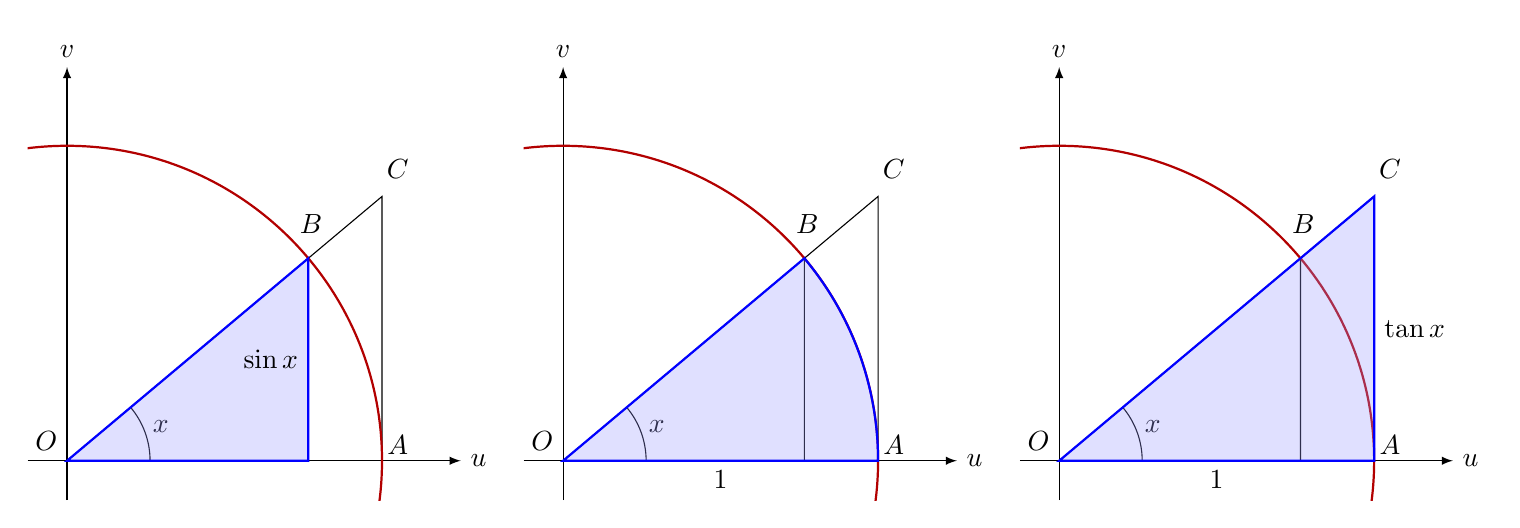
\begin{tikzpicture}[>=latex]
\Base
\filldraw[thick,draw=blue,fill=blue!40,fill opacity=0.3,text opacity=1]
  (O) -- (aux1) -- node[left] {$\sin x$} (aux2)  -- cycle; 

\Base[6.3cm]
\filldraw[thick,draw=blue,fill=blue!40,fill opacity=0.3,text opacity=1]
  (O) -- (aux1) arc (40:0:4) -- node[below] {$1$} cycle; 

\Base[12.6cm]
\filldraw[thick,draw=blue,fill=blue!40,fill opacity=0.3,text opacity=1]
  (O) -- (aux3) -- node[right] {$\tan x$} (aux3|-0,0)  -- node[below] {$1$} cycle; 
\end{tikzpicture}
\vspace{.1cm}
Luego, comparando las areas, $\overset{\triangle}{AOB} <$ \'area sector circular $AOB < \overset{\triangle}{AOC}$.\\
Puesto en valores queda: $\dfrac{|\sin x|}{2} < \dfrac{|x|}{2} < \dfrac{|\tan x|}{2}$ e inmediatamente implica el enunciado.\\

\noindent \textbf{Nota}: La desigualdad $|\sin x| < |x|$ es cierta $\forall x \not = 0$. $|\sin x| \leq 1 < \dfrac{\pi}{2} \leq |x|$\\

\noindent Podemos asegurar tambi\'en que $\displaystyle{\lim_{x\to 0} \sin x} = 0$, pues $0<|x|<\delta \Rightarrow |\sin x| < |x| < \delta < \epsilon$\\

\noindent Tambi\'en es \'util ver que:
\begin{align*}
\cos x &= \cos \left(2\dfrac{x}{2}\right) = \cos\left(\dfrac{x}{2} + \dfrac{x}{2}\right) = \left(\cos \dfrac{x}{2} \cdot \cos \dfrac{x}{2} - \sin \dfrac{x}{2} \cdot \sin \dfrac{x}{2}\right)\\
& = \cos^2 \left(\dfrac{x}{2}\right) - \sin^2 \left(\dfrac{x}{2}\right) = 1 - \sin^2 \left(\dfrac{x}{2}\right) - \sin^2 \left(\dfrac{x}{2}\right) = 1 - 2\cdot \sin^2 \left(\dfrac{x}{2}\right)
\end{align*}
De esta manera podemos concluir que:
$$\lim_{x\to 0}\cos x = \lim_{x\to 0}\left(1 - 2\cdot \sin^2 \left(\dfrac{x}{2}\right)\right) = 1$$

\noindent \textbf{Teorema 8}: Para $a \in \mathbb{R}$:
$$\lim_{x\to a}\sin x = \sin a \ \ \ \ \land \ \ \ \ \lim_{x\to a}\cos x = \cos a$$
\noindent \textbf{Demostraci\'on}: Usando lo anterior m\'as las siguientes formulas:
\begin{itemize}
\item $\displaystyle{\lim_{x\to a}(\sin x) = \lim_{x\to 0} (\sin(x+a)) = \lim_{x\to 0} (\sin x \cdot \cos a + \cos x \cdot \sin a) = 0 \cdot \cos a + 1 \cdot \sin a = \sin a}$
\item $\displaystyle{\lim_{x\to a}(\cos x) = \lim_{x\to 0} (\cos(x+a)) = \lim_{x\to 0} (\cos x \cdot \cos a - \sin x \cdot \sin a) = 1 \cdot \cos a - 0 \cdot \sin a = \cos a}$
\end{itemize}

\noindent \textbf{Corolario 2}: 
\begin{enumerate}
\item Para $a \not = \left(\dfrac{\pi}{2} + k\cdot \pi\right), k \in \mathbb{Z} : \ \ \ \ \displaystyle{\lim_{x\to a} \tan x = \tan a \ \ \ \ \land \ \ \ \ \lim_{x\to a}\sec x = \lim_{x\to a}\dfrac{1}{\cos x} = \dfrac{1}{cos a} = \sec a}$
\item Para $a \not = k\cdot \pi, k \in \mathbb{Z} : \ \ \displaystyle{\lim_{x\to a}\csc x = \lim_{x\to a}\dfrac{1}{\sin x} = \dfrac{1}{\sin a} = \csc a \ \ \land \ \ \lim_{x\to a}\cot x = \lim_{x\to a}\dfrac{\sin x}{\cos x} = \dfrac{\sin a}{\cos a} = \cot a}$\\ \\
\QEDA
\end{enumerate}

\section{El Principio de Intercalaci\'on}
\noindent \textbf{Teorema 9}: \textbf{El Principio de Intercalaci\'on}: Sean $f,g,h$ tres funciones y $a$ un real, tales que en alg\'un entorno reducido $E'(a, \rho)$ se tiene: $g(x) \leq f(x) \leq h(x)$,\\
y adem\'as las funciones $g$ y $h$ tienen l\'imite en $a$ siendo $\displaystyle{\lim_{x\to a} g(x) = \lim_{x\to a} h(x) = l}$,\\
Entonces $f$ tiene l\'imite en el punto $a$ y vale $\displaystyle{\lim_{x\to a} f(x)=l}.$\\
\noindent \textbf{Demostraci\'on}: Tenemos $0<|x-a|<\delta_1 \Rightarrow|g(x)-l| < \epsilon \ \ \land \ \ 0<|x-a|<\delta_2 \Rightarrow |h(x) - l| < \epsilon$\\
Entonces para $\delta = \min\{\rho, \delta_1, \delta_2\}$, y $x$ tal que:
\[0 < |x-a| < \delta \left\{\begin{array}{l}
g(x) \leq f(x) \leq h(x)\\
l - \epsilon < g(x)\\
h(x) < l + \epsilon
\end{array}\right. \Rightarrow (l - \epsilon < f(x) < l + \epsilon) \Rightarrow (|f(x) - l| < \epsilon)\]\\

\noindent \textbf{Proposici\'on 5}: El Principio de Intercalaci\'on es valido si se reemplaza $x\rightarrow a$ por $x\rightarrow a^+$ o $x\rightarrow a^-$.

\noindent \textbf{Proposici\'on 6}: $\displaystyle{\lim_{x \to 0} \dfrac{\sin x}{x} = 1}$\\
\noindent \textbf{Demostraci\'on}: Para $-\dfrac{\pi}{2} < x < \dfrac{\pi}{2}, x \not = 0$, tenemos que $|\sin x| < |x| < |\tan x|$\\
Para los $x$ tales que $0 < x < \dfrac{\pi}{2}$, si dividimos por $\sin x > 0$, tenemos $1 < \dfrac{x}{\sin x} < \dfrac{1}{\cos x}$\\
Para los $x$ tales que $\dfrac{\pi}{2} < x < 0$, si dividimos por $-\sin x > 0$, tenemos $1 < \dfrac{x}{\sin x} < \dfrac{1}{\cos x}$\\
Y como sabemos que $\displaystyle{\lim_{x \to 0} \cos x = 1} \not = 0 \Rightarrow \displaystyle{\lim_{x \to 0} \dfrac{1}{\cos x} = 1}$\\
Utilizando el Teorema del Sandwich, se concluye que $\displaystyle{\lim_{x \to 0} \dfrac{x}{\sin x} = 1 \not = 0}$ y luego $\displaystyle{\lim_{x \to 0} \dfrac{\sin x}{x} = 1}$
\QEDA\\


\end{document}